\section{Automatický plánovač}
\label{sec:planner}

Automatický plánovací systém je implementován jako samostatná aplikace, která podle příchozích požadavků na plánování vytváří
plány. Tyto požadavky přijímá pomocí fronty zpráv RabbitMQ. Plánovač je implementován v jazyce TypeScript a běží v prostředí Node.js.
Pro přístup k databázi využívá stejně jako webová aplikace knihovnu Prisma.

Na základě analýzy fungování plánovače v~původním řešení bylo zjištěno, že plánovač generuje částečně náhodné plány, kterým následně přiřazuje
bodovou penalizaci za nesplněná kritéria. Po uplynutí časové lhůty (přibližně 45 sekund) dojde k ukončení plánování
a je vybrán plán s nejnižší penalizací. Plánovač pracuje s velkým množstvím kritérií a jejich nesplnění vede k rozdílným penalizacím.
Tento postup je neefektivní, protože plánovač musí vygenerovat velké množství plánů, aby
nalezl plán, který splňuje všechna kritéria. Jedná se o výpočetně i časově náročný proces, který je navíc závislý na náhodě.

\subsection{Plánovací algoritmus}

Nové řešení plánovače má v porovnání s původním plánovačem zjednodušený algoritmus s menším množstvím kritérií.
Plánovač vytváří jeden plán na základě požadavků z analýzy v následujících krocích:

\begin{enumerate}
    \item \textbf{Tvorba minimálního plánu:} V prvním kroku plánovač vytvoří minimální korektní plán.\ 
    Plánovač přiřadí ke každé práci požadované minimum silných pracantů, normálních pracantů, pokusí se najít sdílenou jízdu s dříve naplánovanou prací,\ 
    popř. přiřadí řidiče, určí zodpovědného pracanta. Po skončení tohoto kroku jsou všechny joby naplněny do minima. 
    \item \textbf{Doplnění pracantů:} Všechny naplánované joby jsou následně doplněny na maximální možný počet pracantů, kterého je možné dosáhnout bez přidávání řidičů.\ 
    Pracanti s autem nejsou v tomto kroku přiřazováni.
    \item \textbf{Doplnění řidičů:} Joby jsou seřazeny podle počtu chybějících pracantů do maximální kapacity jobu sestupně.\ 
    Do jobů se přiřazují zbylí volní řidiči, pokud jsou na jobu alespoň dvě volná místa. Pokud jsou v jobu pracanti, kteří mají naplánovanou\ 
    sdílenou dopravu s řidičem z jiného jobu, jsou ze sdílené dopravy odebráni a přidáni do auta nově přiřazeného řidiče. Tím může dojít k uvolnění míst v autě jiných jobů.
    \item \textbf{Doplnění pracantů znovu:} V posledním kroku jsou znovu doplněni pracanti do jobů, které nejsou naplněny na maximální kapacitu a mají volná místa v dopravě.
\end{enumerate}

V krocích, kdy dochází k přiřazování pracantů, jsou vybírání pouze pracanti, kteří nejsou alergičtí na alergeny vyskytující se na místě.
V průběhu přiřazování plánovací systém eviduje, zda je v dané oblasti možné adorovat, a pokud ano, snaží se přiřadit pracanta, který projevil zájem o adoraci.
Pokud v oblasti adorovat není možné, přiřazují se pracanti, kteří nevyjádřili zájem o adoraci.
V některých případech není možné vytvořit bezchybný plán -- například není v oblasti adorace dostatek pracovních míst, není dostatek řidičů nebo pracantů na zaplnění
minimálních kapacit všech jobů. V takovém případě plánovač tvoří plán, který je co nejblíže požadovaným kritériím.
Diagram prvního kroku plánovače je zobrazen na obrázku \ref{fig:planner-diagram}.

Toto řešení je výrazně efektivnější než původní řešení, protože plánovač vytváří pouze jeden plán, který v optimálním případě splňuje všechna kritéria.
Během experimentálního testování byl čas potřebný k naplánování úlohy pro obvyklý počet pracantů a jobů v řádu jednotek sekund.

\begin{figure}[h]
    \centering
    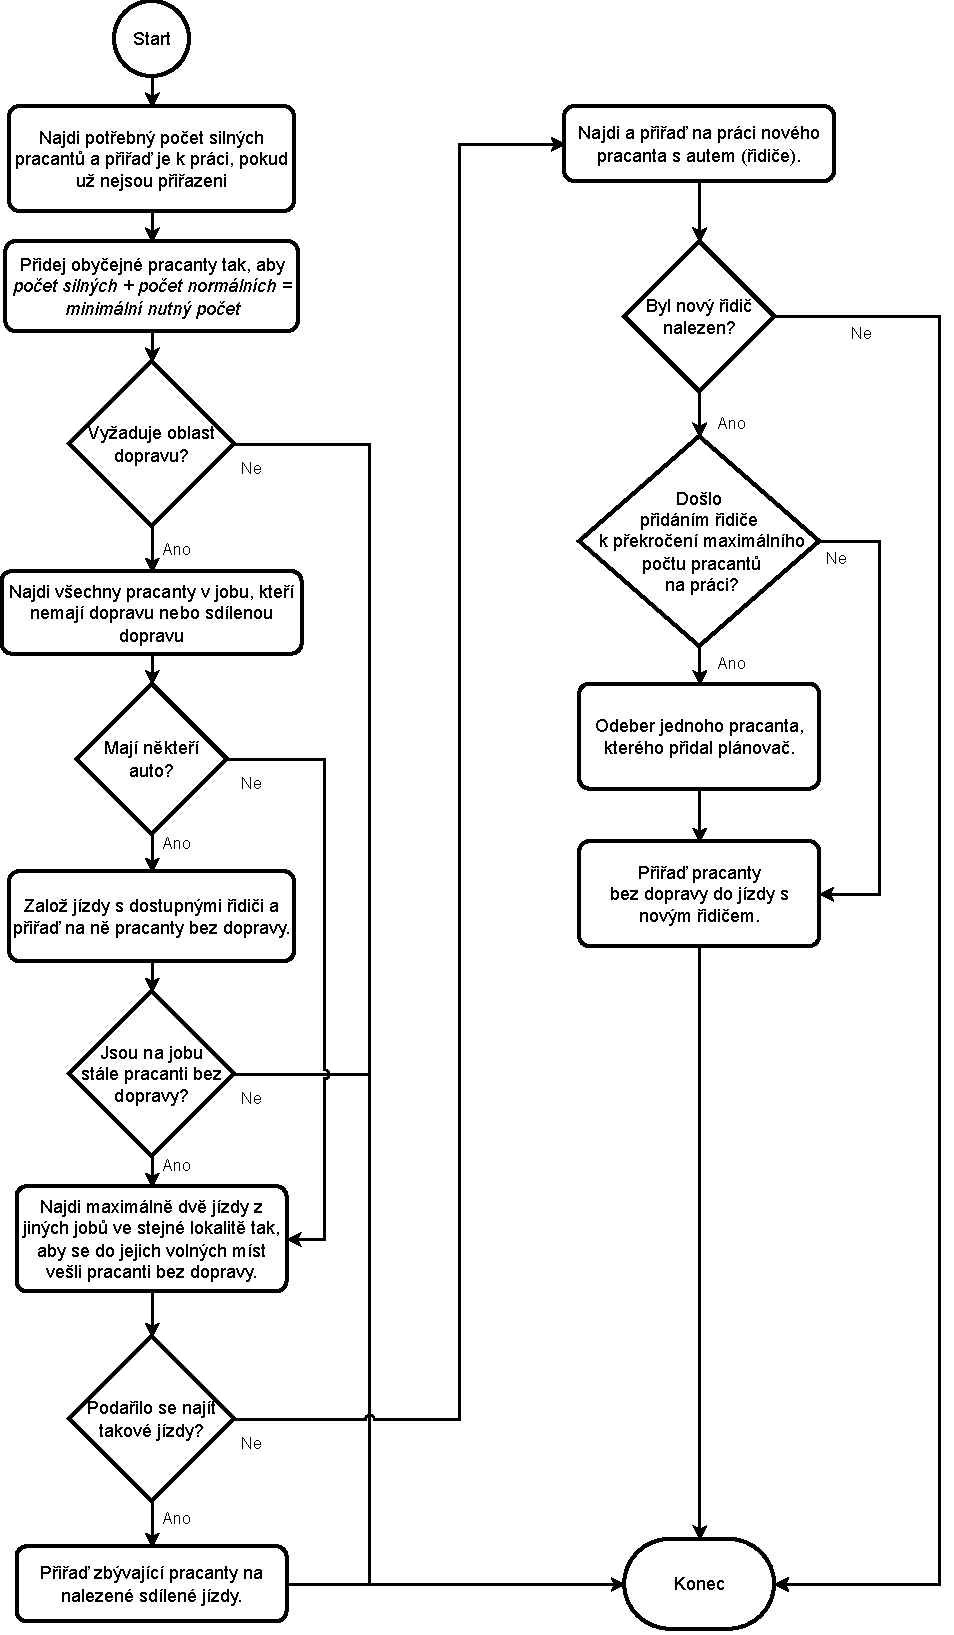
\includegraphics[width=0.9\textwidth]{chapters/images/planner-diagram.pdf}
    \caption{Diagram prvního kroku plánovače pro jednu práci}
    \label{fig:planner-diagram}
\end{figure}


\subsection{Možnosti rozšíření}

Plánovač je navržen tak, aby bylo možné ho rozšířit o další plánovací strategie a kritéria. Třídy pro získávání dat z databáze, ukládání hotových plánů
a komunikaci s frontou zpráv jsou od plánovače odděleny a samotný plánovač implementuje obecné rozhraní. Je tedy možné vytvořit novou třídu, která bude
implementovat rozhraní plánovače a bude obsahovat novou plánovací strategii.

Mezi možná rozšíření plánovače patří například plánování s evidencí nářadí a nástrojů potřebných pro vykonání práce nebo umístění pracantů tak,
aby nebyli opakovaně přiřazováni na stejná místa několika během po sobě následujících dní. Komponentu plánovače je také možné zcela nahradit
jiným plánovacím systémem, který bude komunikovat pomocí fronty zpráv. Takový plánovač může být napsán v jiném programovacím jazyce, pokud by bylo 
například nutné zvýšit výkon nad rámec možností Node.js.
